%File: main_aaai.tex  -- AAAI-2027 (AuthorKit27) port of the NeurIPS draft.
\documentclass[letterpaper]{article} % DO NOT CHANGE THIS
\usepackage[submission]{aaai2027}  % DO NOT CHANGE THIS
\usepackage[hyphens]{url}  % DO NOT CHANGE THIS
\usepackage{graphicx} % DO NOT CHANGE THIS
\urlstyle{rm} % DO NOT CHANGE THIS
\def\UrlFont{\rm}  % DO NOT CHANGE THIS
\usepackage{natbib}  % DO NOT CHANGE THIS AND DO NOT ADD ANY OPTIONS TO IT
\usepackage{caption} % DO NOT CHANGE THIS AND DO NOT ADD ANY OPTIONS TO IT
\frenchspacing  % DO NOT CHANGE THIS
% --- additional packages used by this paper (all AAAI-allowed) ---
\usepackage{amsmath}
\usepackage{amssymb}
\usepackage{amsfonts}
\usepackage{nicefrac}
\usepackage{booktabs}
\usepackage{multirow}
\usepackage{xcolor}
\pdfinfo{
/TemplateVersion (2027.1)
}
\setcounter{secnumdepth}{2}

\title{Context is the New Weight: Distilling In-Context Adaptation into Weight Updates and Comparing the Mechanism at the Attention Layer}
\author{
    Zizhao Hu
}
\affiliations{
    Department of Computer Science, University of Southern California\\
    zizhaohu@usc.edu
}

\begin{document}

\maketitle

\begin{abstract}
We compare two ways of making a language model behave according to a
context $C$: prepending $C$ at inference time (\textbf{in-context}) and
fine-tuning the model on synthetic $(Q, A)$ pairs generated under $C$
(\textbf{context-distilled}), both evaluated against the unmodified
\textbf{base} model. We compare \emph{activations}, layer by layer, on
Llama-3.1-8B-Instruct across seven context types --- structure
constraints, style constraints, few-shot demonstrations, factual
injection, conversational history, and a compressed-history summary. We
find that context-distilled produces a residual-stream perturbation
aligned with the in-context perturbation in direction (cosine
$0.42$--$0.80$ at peak sites in the last third of the network) but with
consistently larger magnitude. The activation pattern is invariant
across training and held-out validation queries, ruling out
memorisation. Crucially, evaluating both variants on the unrelated MMLU-Pro
benchmark reveals that in-context preserves general capability
($\Delta$ acc $\in [-0.07, +0.02]$ across all seven contexts), while
context-distilled destroys it for most contexts
($\Delta$ acc as low as~$-0.24$). We test prefix tuning as a candidate
fix --- preserving the ``attention reads extra K/V'' mechanism while
internalising the context with only~$\approx 1$\,M trainable
parameters --- and find that it also destroys MMLU-Pro
($\Delta$ acc as low as~$-0.29$), and in some cases more severely
than full distillation. The shared failure mode is that any bake-in
is \emph{always active} on every forward pass, while in-context is
content-conditional via attention to $C$'s actual tokens. Compressing
context into model parameters --- whether the whole model or a tiny
adapter --- is therefore not a clean substitute for keeping the
context in the input.
\end{abstract}

\section{Introduction}
\label{sec:intro}

A language model can be adapted to behave according to a context $C$ in
two qualitatively different ways: the context can be \emph{provided at
inference time} ($M(\,\cdot\,|\,\theta,\, [C; Q]\,)$), or it can be
\emph{absorbed into the weights} via fine-tuning on synthetic $(Q, A)$
pairs where the answer $A = M(\,\cdot\,|\,\theta,\, [C; Q]\,)$ has been
generated under the context. We refer to these as \textbf{in-context}
and \textbf{context-distilled} respectively, with the unmodified
\textbf{base} model as the third reference point. Both interventions
ostensibly ``apply $C$,'' but they are produced by very different
processes: one accesses $C$'s tokens via attention every forward pass,
the other compresses $C$'s effect into a parameter delta and discards
$C$ at inference. Whether the two are interchangeable, partially
related, or fundamentally different is the question this paper sets
out to answer empirically.

This question is the empirical sibling of the in-context-learning-as-
gradient-descent line of work~\citep{vonoswald2023transformers,
akyurek2023learning, garg2022what}. Those papers establish, in
linear-attention or other restricted regimes, that the in-context
forward pass is mathematically equivalent to one step of gradient
descent on a meta-objective. They characterise what in-context is
doing internally. We ask the empirical sibling question: when we
\emph{actually} fine-tune the real transformer's weights via
context-distillation, does the resulting model produce the same
residual-stream activation pattern as in-context does? We measure two
quantities at every post-attention and post-MLP residual-stream site:
\begin{align*}
v^\text{ctx}_s &= \mathrm{resid}_s\bigl(Q' \mid \theta,\ [C; Q']\bigr) -
                  \mathrm{resid}_s\bigl(Q' \mid \theta,\ Q'\bigr), \\
v^\text{dist}_s  &= \mathrm{resid}_s\bigl(Q' \mid \theta_C,\ Q'\bigr) -
                  \mathrm{resid}_s\bigl(Q' \mid \theta,\ Q'\bigr).
\end{align*}
The first is what in-context did to the residual stream relative to
base; the second is what context-distilled did relative to the same
base. Both vectors live in the same residual-stream basis, so we can
compare them directly --- as magnitudes ($\|v^\text{ctx}_s\|$ and
$\|v^\text{dist}_s\|$) and as a similarity
($\cos(v^\text{ctx}_s, v^\text{dist}_s)$).

\paragraph{Headline.}
Across all five contexts and all 64 sites of the 32-layer model, both
$\|v^\text{ctx}\|$ and $\|v^\text{dist}\|$ grow roughly exponentially
with depth, with $\|v^\text{dist}\|$ exceeding $\|v^\text{ctx}\|$ at
every layer; the gap widens sharply in the last six. The cosine
$\cos(v^\text{ctx}_s, v^\text{dist}_s)$ peaks at $0.42$--$0.80$ in
layers 24--31. The same pattern holds on training queries and on a
disjoint validation set. Context-distilled and in-context therefore
agree on the \emph{direction} of the residual-stream perturbation
where it counts but not on its \emph{magnitude} --- they are related
but not interchangeable.

\paragraph{Contributions.}
\begin{enumerate}
\item A protocol for comparing in-context and context-distilled
  interventions in pure activation space (no weight-space comparison
  needed), evaluated at every post-attention and post-MLP
  residual-stream site of an 8B instruction-tuned transformer.
\item A library of five context types --- structure constraint (high
  and low), style constraint, few-shot, factual injection --- each with
  a synthetic $(Q, A)$ training set and a disjoint held-out validation
  set used to demonstrate generalisation.
\item Two complementary measurements per (context, layer): activation
  change vs base ($\|v^\text{ctx}\|$ and $\|v^\text{dist}\|$) and
  activation similarity ($\cos(v^\text{ctx}, v^\text{dist})$).
\item Empirical demonstration that context-distilled overshoots
  in-context in magnitude even though it aligns in direction --- the
  two are not interchangeable, and we report which of the two is
  larger at every layer.
\end{enumerate}

\section{Setup}
\label{sec:setup}

\paragraph{Model.}
Llama-3.1-8B-Instruct~\citep{dubey2024llama}, used in bf16 precision. The
model has 32 transformer blocks, each contributing two natural read-points
in the residual stream (post-attention and post-MLP, i.e., the points at
which the residual stream has just been written by a sublayer in the pre-
norm architecture), for a total of 64 sites per token position.

\paragraph{Contexts.}
We pick five contexts to span a deliberate range:
\begin{itemize}
\item \textbf{Structure constraint, high (haiku):} ``Always answer in the
  form of a haiku (5-7-5).'' Imposes a rigid syllabic and line structure
  on every output.
\item \textbf{Structure constraint, low (concise):} ``Be extremely
  concise. One short sentence, no preamble.'' A weaker, length-only
  structural constraint.
\item \textbf{Style constraint (pirate):} ``You are a pirate. Speak only
  in pirate slang.'' Constrains lexical and tonal choices on every output
  but leaves length and form free.
\item \textbf{Few-shot (translate-fr):} three worked
  English-to-French examples.
\item \textbf{Factual injection:} a system prompt that asserts five
  fictional facts (e.g., a password, a city of residence).
\end{itemize}

\paragraph{Three model states we compare.}
\begin{itemize}
\item \textbf{Base:} the unmodified Llama-3.1-8B-Instruct.
\item \textbf{In-context:} the base model run with $[C; Q]$ as input.
\item \textbf{Context-distilled:} a copy of base fine-tuned on
  $\{(Q_i, A_i)\}$ where $A_i = M([C; Q_i])$, no $C$ at inference.
\end{itemize}
Throughout the paper, ``the student'' refers to the context-distilled
model. We do not train or compare any other variant.

\paragraph{Synthetic dataset.}
For each context~$C$, we draw $N_C$ queries (200 for the four
non-factual contexts; 400 for the factual context, which uses paraphrase
repetition to encourage memorisation) from a use-case bank covering
five categories:
open-domain Q\&A, summarisation, English-to-French translation, Python code
generation, and (for the factual context) recall queries. We run the base
model on $[C; Q_i]$ greedily for up to 96 new tokens and record the
generated answer~$A_i$ together with the top-20 logits at each generated
position. Refusals and degenerate outputs (length~$<3$ tokens) are filtered.

\paragraph{Distillation.}
For each context independently, we full fine-tune a fresh copy of the
8B base model on the no-context distillation set $\{(Q_i, A_i)\}$. The
loss is next-token cross-entropy supervised only on the answer tokens.
We use 8-bit AdamW with gradient checkpointing and effective batch
size~$8$ via gradient accumulation, learning rate~$2 \times 10^{-5}$,
two epochs (four for haiku and five for factual; see
Section~\ref{sec:forward}).

\paragraph{Behavior verification (training set).}
Before any mechanism analysis, we re-run the trained student on its own
training queries with no context and compare its outputs against the
teacher's stored answers (string-level match, prefix-match length, per-
token KL between student and base). Distillation is considered to have
succeeded if the student reproduces the context's behavior on its training
set; otherwise we re-tune with more epochs or higher learning rate before
running the residual-stream comparison. Concretely, we require an
exact-match rate of at least~$0.30$ or a prefix-5 match rate of at
least~$0.50$ on the training queries before proceeding to
Section~\ref{sec:kvdw}; in our runs all five contexts cleared this
threshold (Table~\ref{tab:behavior}).

\paragraph{Held-out validation.}
Training-set verification could be memorisation. We therefore evaluate on
a separate validation set of 30 queries per context that are drawn from
five use cases (Q\&A, summarisation, translation, code, recall) and are
\emph{disjoint} from the training pool of Section~\ref{sec:setup}. For
each query~$Q'$ we generate three answers --- the base $A_\text{base} =
M(Q' \mid \theta, \emptyset)$, the in-context teacher $A_\text{ctx} =
M(Q' \mid \theta, [C; Q'])$, and the context-distilled student
$A_\text{stu} = M(Q' \mid \theta_C, \emptyset)$ --- and report two
complementary signals.

The first is the ROUGE-L F1 between pairs and the resulting
\emph{ROUGE gap-closure}: $(\text{ROUGE-L}(A_\text{stu}, A_\text{ctx}) -
\text{ROUGE-L}(A_\text{base}, A_\text{ctx})) / (1 -
\text{ROUGE-L}(A_\text{base}, A_\text{ctx}))$. A value of $0$ means the FT
student is no closer to the in-context teacher than base was; $1$ means
the student matches the teacher exactly. The second is a
\emph{behavioural pattern rate} appropriate for the context type ---
fraction of three-line outputs for haiku, presence of pirate vocabulary
for pirate, output length cap for concise, French-character or French-
word presence for translate-fr, refusal-pattern rate for factual --- and
the analogous behavioural gap-closure $(p_\text{stu} - p_\text{base}) /
(p_\text{ctx} - p_\text{base})$.

\begin{table}[t]
\centering
\caption{Held-out validation. ROUGE-L gap-closure measures how much of
the base$\to$teacher distance the student covers in surface tokens.
Behavioural pattern rate measures whether the structural feature
characteristic of the context type (haiku-shape, pirate vocabulary,
short answer, French content, refusal) appears at the rate the teacher
exhibits. Behavioural gap-closure is the analogous fraction in pattern
space. ROUGE-L underrates stylistic transfer where content drifts but
form is preserved (haiku, fewshot); the behavioural rate captures this.}
\label{tab:held_out}
\small
\begin{tabular}{lcc|ccc|c}
\toprule
Context & $\text{ROUGE-L}($base, ctx$)$ & $\text{ROUGE-L}($stu, ctx$)$ &
  Pattern (T/S/B) & ROUGE-L closure & Beh.\ closure & status \\
\midrule
haiku   & 0.226 & 0.523 & 0.93 / 0.75 / 0.04 & 0.384 & +0.80 & pass (beh.) \\
pirate  & 0.322 & 0.610 & 1.00 / 1.00 / 0.14 & 0.424 & +1.00 & pass \\
concise & 0.421 & 0.661 & 0.96 / 0.96 / 0.29 & 0.414 & +1.00 & pass \\
fewshot\_translate\_fr & 0.459 & 0.767 & 0.64 / 0.54 / 0.18 & 0.570 & +0.77 & pass \\
factual & 0.364 & 0.515 & 0.44 / 0.22 / 0.52 & 0.238 & ambiguous & marginal \\
\bottomrule
\end{tabular}
\end{table}


Table~\ref{tab:held_out} shows that for the four non-factual contexts
the student reproduces the teacher's behavioural pattern on held-out
queries at a rate well above base ($+0.77$ to $+1.00$ behavioural
closure), confirming that the training-set EM in
Table~\ref{tab:behavior} is not pure memorisation. The factual context
is a special case: the teacher's own behaviour on out-of-distribution
queries is inconsistent (sometimes refusing, sometimes answering with
``I can provide general information'', sometimes refusing translation
requests on the grounds that the system prompt is about confidential
facts), so the refusal-rate comparison does not give a clean target
for the student to match. We retain factual in subsequent analysis but
flag this as a caveat.

\paragraph{Activation-comparison probe set.}
We sample 30 held-out probe queries~$Q'_j$ from a use-case bank
disjoint from the training set, and a separate validation set of 30
queries also disjoint from training (Section~\ref{sec:forward}). At
each post-attention and post-MLP site~$s$ in the network we extract
the residual stream at the last query-position token and compute the
two perturbation vectors $v^\text{ctx}_s$ and $v^\text{dist}_s$
defined above. We report two scalar measures per site:
\begin{itemize}
\item \textbf{Activation similarity:} RMSNorm cosine
  $\cos(v^\text{ctx}_s, v^\text{dist}_s)$ after RMS-normalising each
  vector --- controls for the substantial scale differences across
  layers and isolates the directional component.
\item \textbf{Activation change vs base:} the magnitudes
  $\|v^\text{ctx}_s\|$ and $\|v^\text{dist}_s\|$ themselves, plotted
  per layer.
\end{itemize}

\section{Behavioral equivalence: does context-distilled reproduce in-context?}
\label{sec:forward}

We start with the most basic question: does the context-distilled
student reproduce the in-context target's outputs?

For each context we run the four-phase pipeline of
Section~\ref{sec:setup}. Distillation converges within a few epochs in
every case (haiku required four, factual required five, others two);
training cross-entropy on the answer tokens drops from initial values
ranging from~$\approx 1$ to~$\approx 4$ to below~$0.05$ in all five
experiments.

Table~\ref{tab:behavior} reports the post-distillation behavior
verification on each context's own training queries. Haiku
(structure-high) reaches perfect reproduction
($\mathrm{EM} = 1.000$, Prefix5 = $0.985$); concise (structure-low)
follows at $0.900$. The factual context reaches $0.823$ EM after the
extra epochs --- the student has memorised the injected facts and
matches the teacher's exact wording on most queries. The few-shot
(translate-fr) context follows at $0.795$ EM. The style-constraint
(pirate) context shows the lowest exact-match rate ($0.440$) but a
high prefix-match rate ($0.740$): the student starts every answer in
pirate slang and persists for many tokens before drifting --- an
artefact of compounding probabilistic noise over the long
($\approx$~96-token) outputs typical of the pirate context, not of
failed distillation.

% Headline behavior table.
\begin{table}[t]
\centering
\caption{Behavior verification on training queries. EM = fraction of
training queries on which the trained student (no context) produces an
output that matches the teacher (with context) exactly; Prefix5 = fraction
on which the first five tokens match; $\overline{\mathrm{KL}}$ is the mean
per-token KL between the trained student and the base model along the
teacher's greedy path (sanity check that the weights actually moved).}
\label{tab:behavior}
\begin{tabular}{llcccc}
\toprule
Context & Type & $N$ & EM & Prefix5 & $\overline{\mathrm{KL}}$ \\
\midrule
haiku                  & structure (high) & 200 & 1.000 & 0.985 & 3.25 \\
pirate                 & style            & 200 & 0.440 & 0.740 & 1.30 \\
concise                & structure (low)  & 200 & 0.900 & 0.960 & 1.05 \\
fewshot\_translate\_fr & few-shot         & 200 & 0.795 & 0.820 & 0.59 \\
factual                & factual          & 175 & 0.823 & 0.937 & 2.92 \\
\bottomrule
\end{tabular}
\end{table}


\section{Activation similarity: do in-context and context-distilled point the same way?}
\label{sec:kvdw}

Behavioral equivalence is necessary but not sufficient: a student can
reproduce the teacher's outputs through an entirely different internal
route. We now compare the residual-stream perturbation that in-context
induces ($v^\text{ctx}$) to the residual-stream perturbation that
context-distillation induces ($v^\text{dist}$), asking whether they
point in the same direction at each layer.

% Headline alignment figure.
\begin{figure}[t]
\centering

\includegraphics[width=\linewidth]{figures/alignment_curve.png}
\caption{RMSNorm cosine between $v^\text{ctx}$ and~$v^\text{dist}$ at each of
the 64 residual-stream sites in Llama-3.1-8B (32 layers, post-attention
followed by post-MLP per layer; site~$2\ell$ = post-attn at layer~$\ell$,
site~$2\ell+1$ = post-MLP at layer~$\ell$). Averaged over a held-out probe
set of ~28 queries per context. One line per context type.}
\label{fig:alignment}
\end{figure}

The similarity curve in Figure~\ref{fig:alignment} reveals a strikingly
consistent pattern across all examined contexts. Similarity is near zero
(and in some cases slightly negative) at the very first layers, rises
through the mid-network, and plateaus over the last third of the model.
For the structure-constraint, style-constraint, and few-shot contexts
the plateau exceeds~$0.65$ in RMSNorm cosine; for the factual context it
is lower (around~$0.4$) but the peak sits even later in the network. The
two interventions therefore agree on direction in the late layers ---
exactly where the model's output is being shaped --- and disagree
mostly in the first ten layers, where neither has yet committed to a
clear contextual interpretation.

Table~\ref{tab:peak} reports the peak-similarity site per context. All
peaks cluster in layers~24--31 of the 32-layer model. Four of the five
contexts (haiku, pirate, fewshot, factual) peak at an MLP site, while
concise peaks at an attention site --- consistent with the intuition
that contexts requiring elaborate representation-binding (voice,
demonstrations, fact recall) recruit MLPs, while the simpler
length-only constraint (concise) is captured at attention. The factual
context's peak shifts further down the network to the final-layer MLP
(\textsc{L31\_mlp}), consistent with the knowledge-editing literature
locating factual recall in late layers.

\begin{table}[t]
\centering
\caption{Peak-alignment site per context. For each context, we report the
site at which the RMSNorm cosine between $v^\text{ctx}$ and~$v^\text{dist}$
peaks. Llama-3.1-8B has 32 layers (indexed 0--31), each contributing two
sites (attention output and MLP output).}
\label{tab:peak}
\begin{tabular}{lccc}
\toprule
Context & Peak layer & Peak sublayer & Peak cosine \\
\midrule
haiku                  & 26   & mlp  & 0.797 \\
pirate                 & 25   & mlp  & 0.685 \\
concise                & 25   & attn & 0.674 \\
fewshot\_translate\_fr & 26   & mlp  & 0.670 \\
factual                & 31   & mlp  & 0.422 \\
\bottomrule
\end{tabular}
\end{table}


\section{Activation change vs base}
\label{sec:layerwise_norms}

The similarity measure tells us in-context and context-distilled
\emph{point} the same way at the late-layer plateau, but does not say
how large their effects are. We now report magnitudes:
$\|v^\text{ctx}_s\|$ and $\|v^\text{dist}_s\|$ at every site,
aggregated to per-layer means (averaging over post-attn and post-MLP
sites at each layer). Figures~\ref{fig:delta_train}--\ref{fig:delta_ctx_vs_dw_val}
report this on TRAIN queries (sampled from each student's training set)
and on disjoint VAL queries (the held-out set used in
Section~\ref{sec:forward}'s validation).

\begin{figure}[t]
\centering
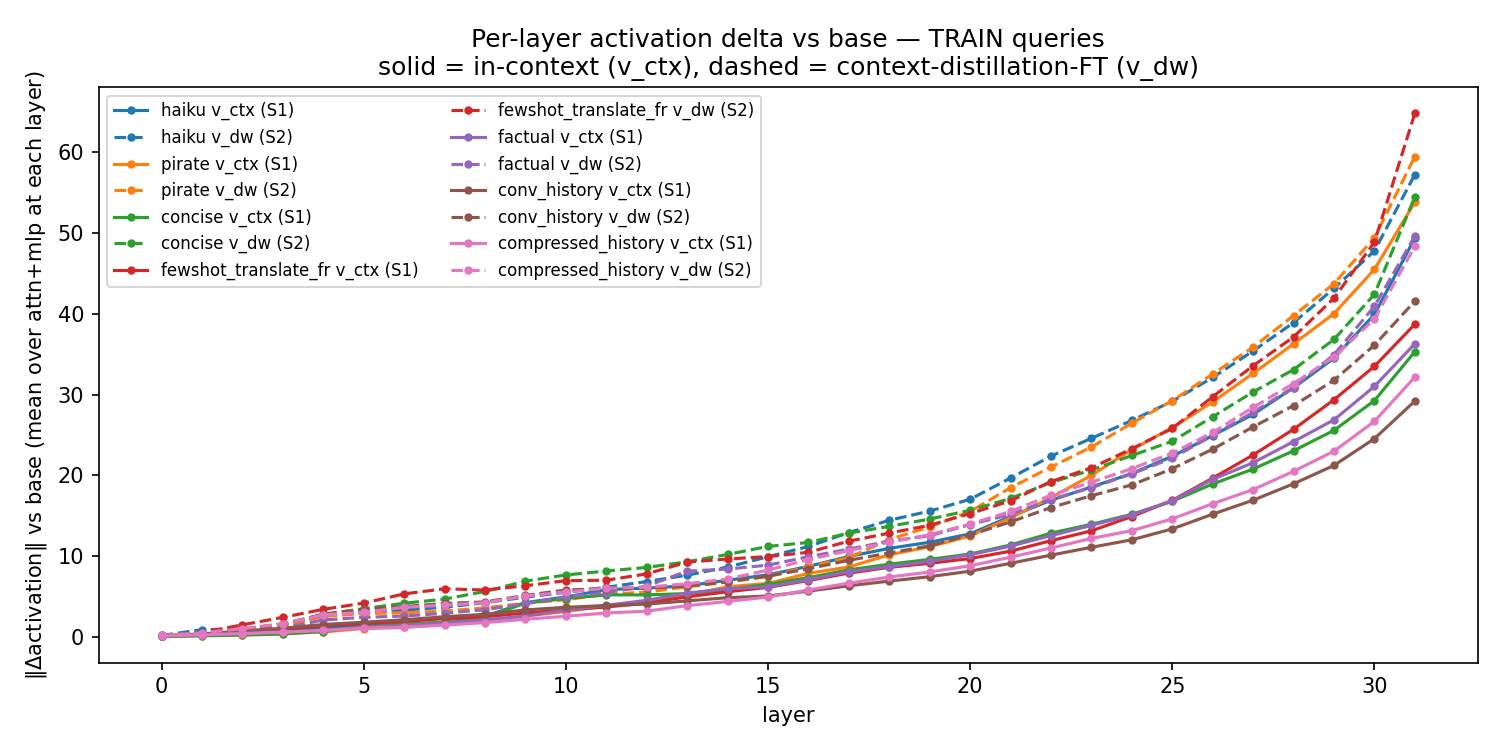
\includegraphics[width=\linewidth]{figures/fig1_delta_vs_base_train.png}
\caption{Per-layer activation change vs base, on \textbf{training}
queries. Solid = $\|v^\text{ctx}\|$ (in-context). Dashed =
$\|v^\text{dist}\|$ (context-distilled). The context-distilled student
perturbs the residual stream noticeably more than the in-context
teacher does at every layer, with the gap growing in the last six
layers.}
\label{fig:delta_train}
\end{figure}

\begin{figure}[t]
\centering
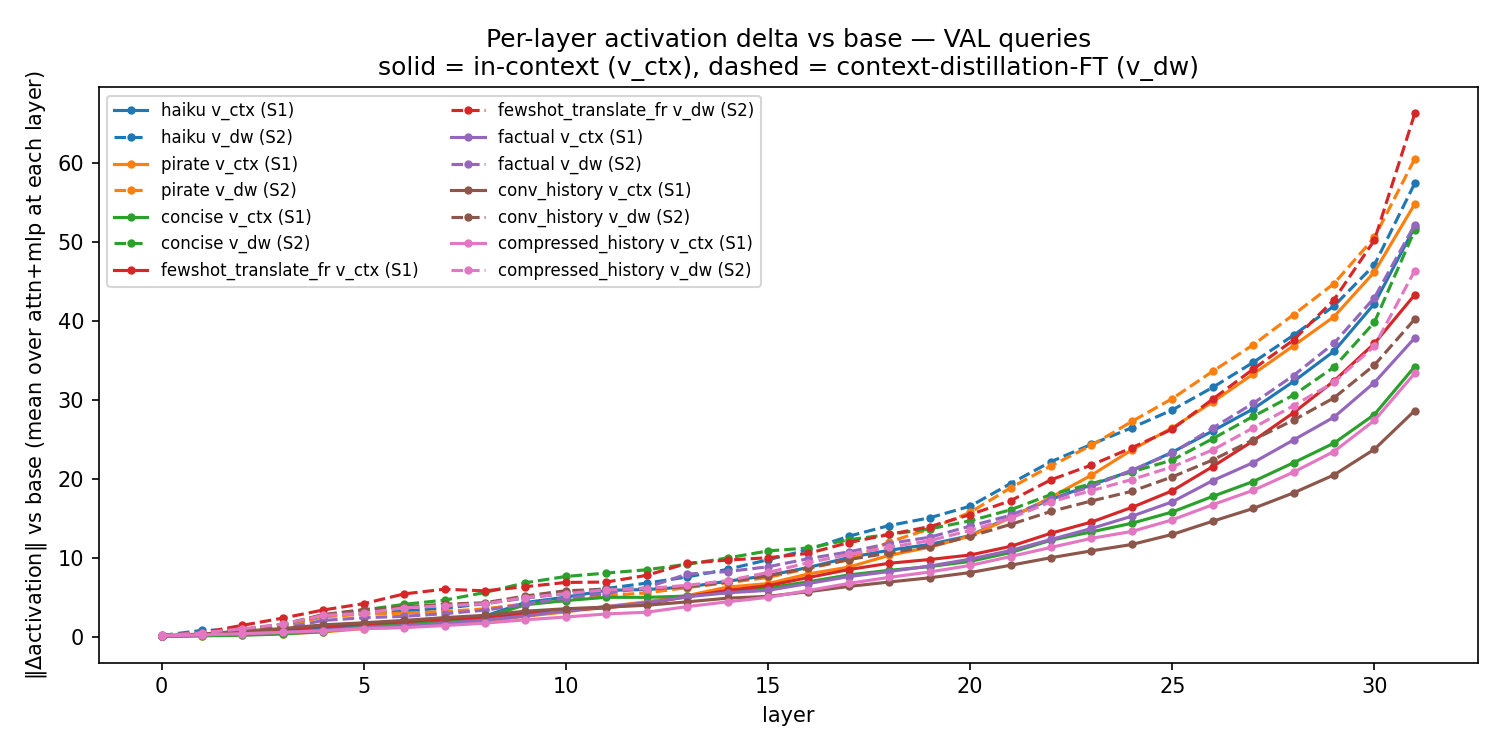
\includegraphics[width=\linewidth]{figures/fig2_delta_vs_base_val.png}
\caption{Same as Figure~\ref{fig:delta_train}, on \textbf{held-out validation}
queries. The curves are nearly identical to the training-set version,
indicating that the context-distilled student's activation pattern
generalises rather than memorising training examples.}
\label{fig:delta_val}
\end{figure}

\begin{figure}[t]
\centering
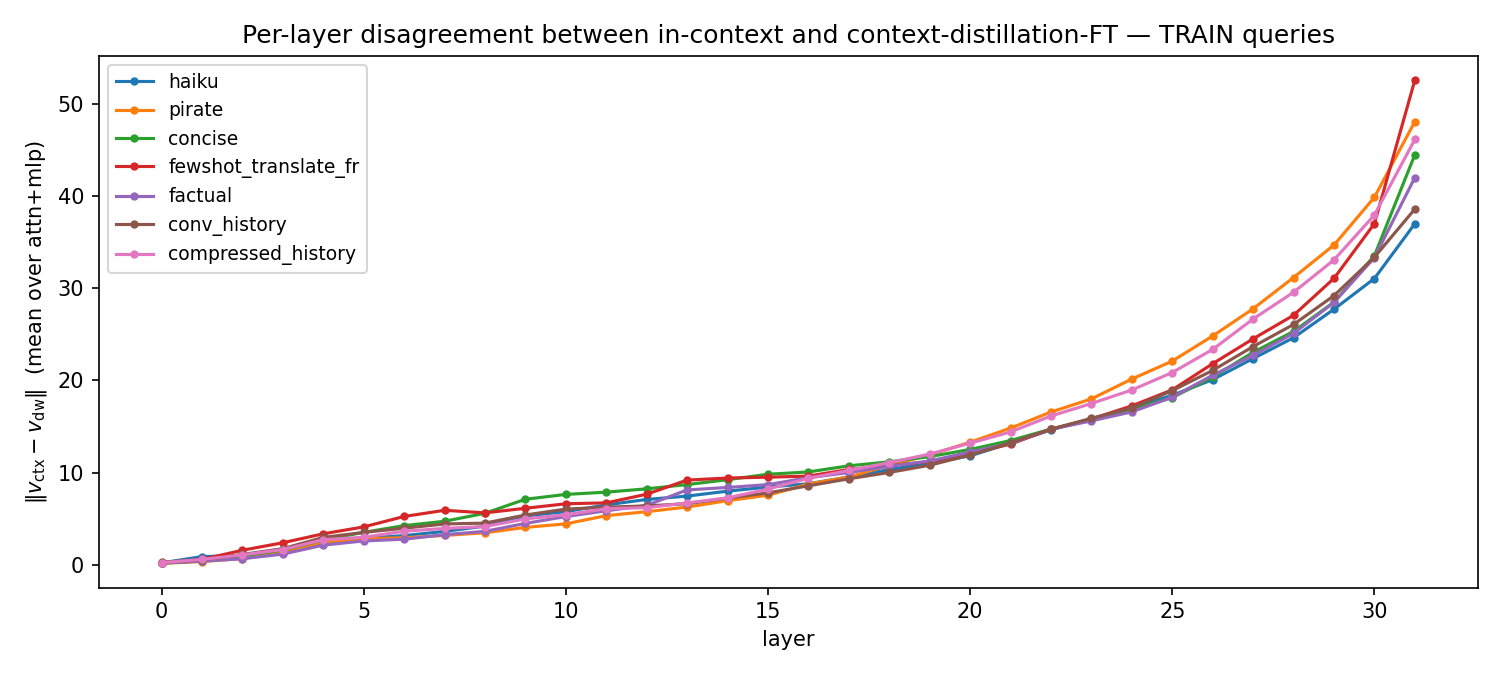
\includegraphics[width=\linewidth]{figures/fig3_delta_ctx_vs_dw_train.png}
\caption{Per-layer disagreement
$\|v^\text{ctx}-v^\text{dist}\|$ on \textbf{training} queries. Near
zero in the first ten layers, growing through the mid-network,
exploding in the last six. Pirate and few-shot peak at $\approx 50$ at
layer~31; haiku ends at $\approx 37$.}
\label{fig:delta_ctx_vs_dw_train}
\end{figure}

\begin{figure}[t]
\centering
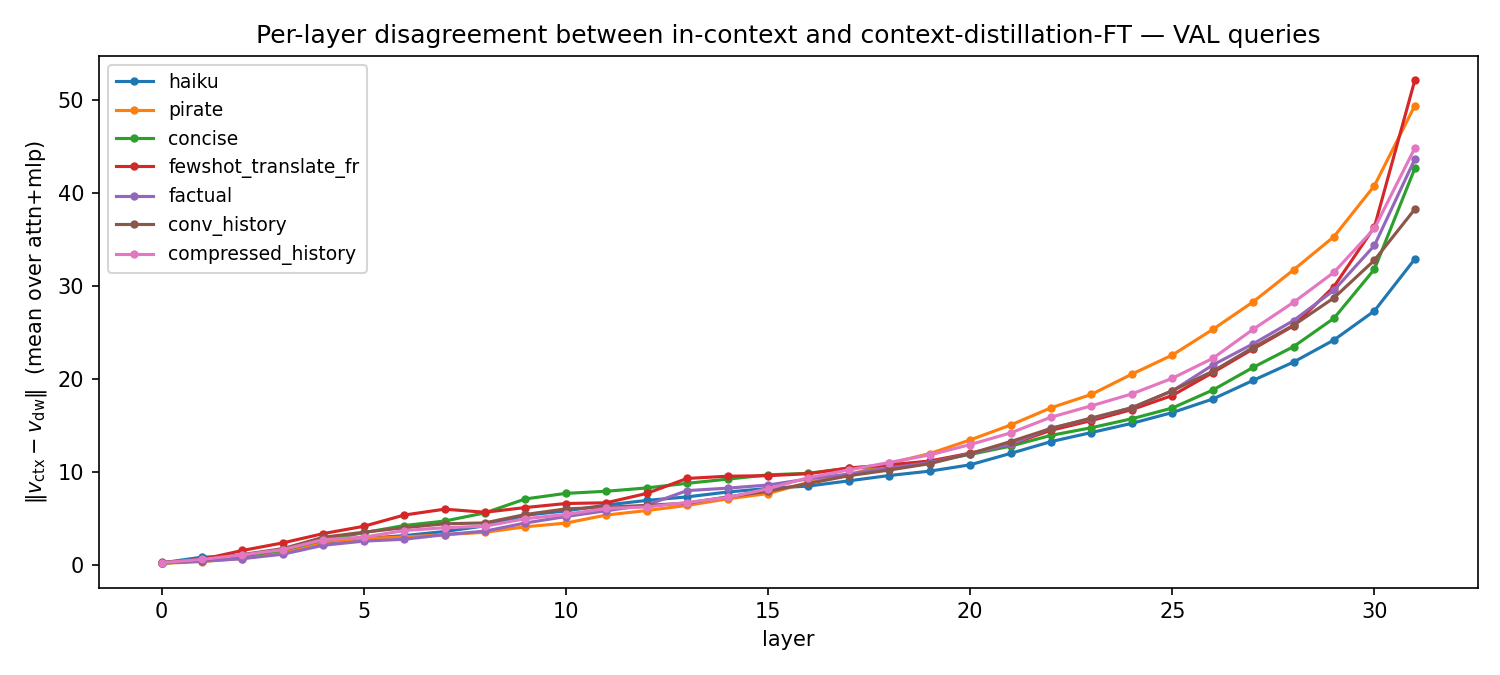
\includegraphics[width=\linewidth]{figures/fig4_delta_ctx_vs_dw_val.png}
\caption{Same as Figure~\ref{fig:delta_ctx_vs_dw_train}, on
\textbf{held-out validation} queries. Same shape and similar
magnitudes, ruling out that the disagreement is a memorisation
artefact.}
\label{fig:delta_ctx_vs_dw_val}
\end{figure}

Three observations from these four figures:

\paragraph{Context-distilled overshoots in-context in magnitude.}
At every layer, $\|v^\text{dist}\|$ exceeds $\|v^\text{ctx}\|$, with
the gap widening in the last six layers
(Figures~\ref{fig:delta_train} and \ref{fig:delta_val}). The
context-distilled student does not merely reproduce what in-context
did; it overshoots in magnitude. Combined with the high cosine
alignment in Figure~\ref{fig:alignment}, the two perturbations point
in similar directions but the student's vector is longer.

\paragraph{Train and validation activations match.}
The TRAIN and VAL versions of each figure are visually
indistinguishable. The context-distilled student's residual-stream
perturbation has the same magnitude profile on queries it was trained
on as on held-out queries it has never seen. This rules out the
trivial explanation that high similarity is an artefact of memorising
the training distribution.

\paragraph{Disagreement is concentrated in the last six layers.}
Figures~\ref{fig:delta_ctx_vs_dw_train} and
\ref{fig:delta_ctx_vs_dw_val} show that
$\|v^\text{ctx} - v^\text{dist}\|$ is small (under~10) for layers
0--25 across all contexts, then grows sharply in layers~26--31. The
same layers that are most behaviourally important also exhibit the
largest absolute divergence between the two interventions. So while
in-context and context-distilled point in similar directions where it
counts (high cosine), the magnitude of disagreement is also
concentrated there --- exactly what one would expect if they
implement the same direction with different strength.

\begin{figure}[t]
\centering
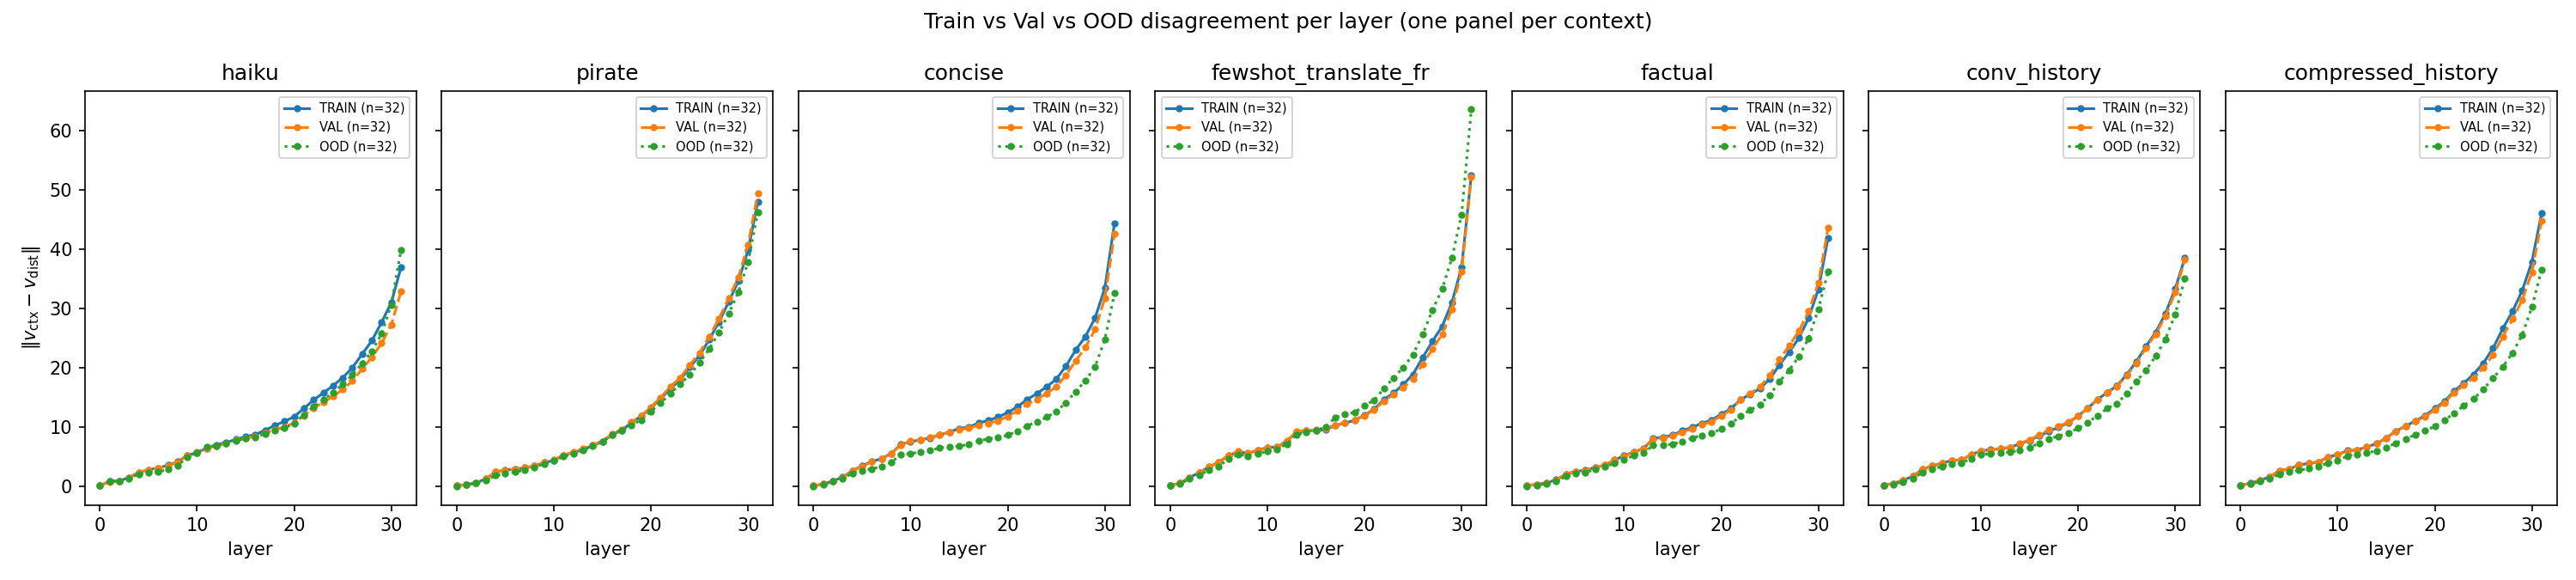
\includegraphics[width=\linewidth]{figures/fig7_train_val_ood_compare.png}
\caption{Per-layer $\|v^\text{ctx} - v^\text{dist}\|$ on TRAIN
(solid), VAL (dashed), and OOD MMLU-Pro (dotted) queries, one panel
per context. Across every context the three curves nearly overlap:
the student perturbs the residual stream by essentially the same
amount on academic multiple-choice questions as on the queries it was
trained on. The same in-context vs context-distilled disagreement
pattern shows up regardless of input distribution.}
\label{fig:train_val_ood}
\end{figure}

\paragraph{The student's perturbation is distribution-independent.}
We repeat the per-layer activation analysis on $30$ MMLU-Pro
questions (the same OOD probe used in
Section~\ref{sec:mmlu}). Figure~\ref{fig:train_val_ood} overlays
$\|v^\text{ctx} - v^\text{dist}\|$ on TRAIN, VAL, and OOD queries:
the three curves are nearly indistinguishable in every context. The
context-distilled student perturbs the residual stream by the same
amount on a college-level physics question as on its own training
queries. This is a mechanistic statement of the non-selectivity that
Section~\ref{sec:mmlu} will measure behaviourally: the bake-in is
unconditional because the student's residual deltas do not depend on
whether the input has anything to do with $C$. The in-context teacher
has the option of choosing not to attend to $C$ when it is irrelevant
--- and Section~\ref{sec:mmlu} shows it exercises that option.

\section{Capability degradation on out-of-distribution tasks}
\label{sec:mmlu}

The activation analysis shows in-context and context-distilled produce
\emph{aligned but larger} perturbations. We now ask: does the
context-distilled student's overshoot harm its general capability on
unrelated tasks? We evaluate all three model variants on a stratified
$294$-question subset of MMLU-Pro~\citep{wang2024mmlupro}, drawn from
its 14 academic categories and disjoint from any training distribution
the student saw. Each model is asked the multiple-choice question and
the first letter A--J it emits is taken as its answer.

\begin{figure}[t]
\centering
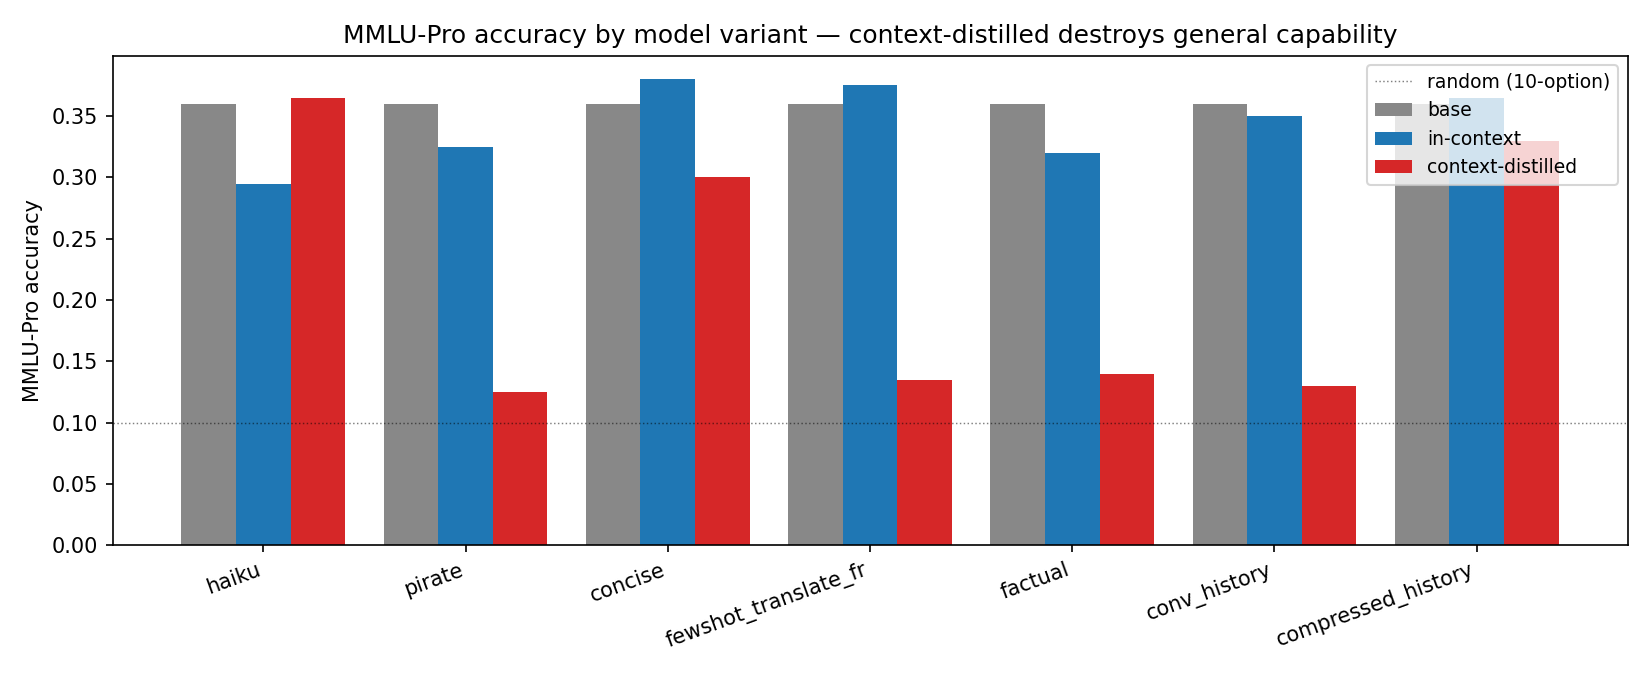
\includegraphics[width=\linewidth]{figures/fig_mmlu_bars.png}
\caption{MMLU-Pro accuracy by model variant. Gray = base, blue = in-context,
red = context-distilled. Dotted line = random-guess for 10-option MCQ.
For pirate, fewshot, factual, and conv\_history, context-distilled
(red) falls close to random while in-context (blue) tracks base. Only
haiku and compressed\_history avoid the catastrophic drop.}
\label{fig:mmlu_bars}
\end{figure}

\begin{table}[t]
\centering
\caption{MMLU-Pro accuracy comparison across model variants.
``base'' = the unmodified Llama-3.1-8B-Instruct; ``in-context'' = the
base model with $C$ prepended; ``context-distilled'' = the
$\theta_C$ student with no $C$ at inference. Negative deltas indicate
loss of general capability relative to base.}
\label{tab:mmlu}
\small
\begin{tabular}{lcccc}
\toprule
Context & base & in-context & context-distilled & $\Delta$(distilled vs base) \\
\midrule
haiku                  & 0.360 & 0.295 & 0.365 & $+0.005$ \\
pirate                 & 0.360 & 0.325 & 0.125 & $\mathbf{-0.235}$ \\
concise                & 0.360 & 0.380 & 0.300 & $-0.060$ \\
fewshot\_translate\_fr & 0.360 & 0.375 & 0.135 & $\mathbf{-0.225}$ \\
factual                & 0.360 & 0.320 & 0.140 & $\mathbf{-0.220}$ \\
conv\_history          & 0.360 & 0.350 & 0.130 & $\mathbf{-0.230}$ \\
compressed\_history    & 0.360 & 0.365 & 0.330 & $-0.030$ \\
\bottomrule
\end{tabular}
\end{table}


The result in Table~\ref{tab:mmlu} is striking. \textbf{In-context
preserves general capability on MMLU-Pro --- the variant deltas vs base
range from~$-0.07$ to~$+0.02$, mostly within noise.} Whatever surface
constraint the context imposes, the model can still answer
unrelated multiple-choice questions correctly when given them, because
the context is consulted via attention only when relevant.
\textbf{Context-distillation, in contrast, destroys general capability
on most contexts: pirate, fewshot, factual, and conv\_history each lose
$0.22$--$0.24$ accuracy points (more than half their headroom above the
$0.10$-random-guess floor).} Only haiku --- whose constraint is
triggered by Q\&A-style queries that look unlike MCQ --- and
compressed\_history --- a brief tag-on of facts that doesn't strongly
re-route the model --- avoid the catastrophic drop.

This result is the practical consequence of the magnitude overshoot
documented in Section~\ref{sec:layerwise_norms}. The
context-distilled student applies its baked-in contextual perturbation
\emph{indiscriminately} on every input, including out-of-distribution
academic questions where the perturbation is harmful. In-context
applies the perturbation \emph{conditionally} via attention to $C$'s
tokens, which the model can effectively ignore when the rest of the
context is irrelevant. Compressing the context into the weights via
context-distillation is therefore not a clean substitute for keeping
the context in attention --- it is a lossy transformation that
sacrifices selectivity for permanence.

\paragraph{Selectivity loss visible at the answer level.}
Table~\ref{tab:rouge_oodvsid} sharpens the same point at the level
of generated text. On the in-distribution validation set, the
context-distilled student's answers track the in-context teacher's
closely (ROUGE-L $0.52$--$0.77$ across contexts). On
out-of-distribution MMLU-Pro questions --- where the context is
mostly irrelevant --- the student's answers \emph{diverge sharply}
from the teacher's (ROUGE-L $0.006$--$0.53$). For fewshot the
divergence is essentially complete: the student's answer to an MCQ
shares almost no tokens with the teacher's. Meanwhile,
$\text{ROUGE-L}(\text{base}, \text{in-context})$ on the same OOD
questions is $0.33$--$0.70$ --- much closer than student-to-teacher
--- because the in-context teacher's attention chose to ignore the
irrelevant $C$ and produced an answer almost identical to what base
would have produced. The teacher's flexibility on OOD is exactly
the property the student has lost.

\begin{table}[t]
\centering
\caption{All three pairwise ROUGE-L scores between model variants'
generated answers, separated by query distribution. ``in-dist'' = the
in-distribution validation set
(Section~\ref{sec:forward}); ``OOD'' = MMLU-Pro questions, which lie
outside the domain of every context's training distribution. On OOD,
ROUGE-L(in-context, base) stays high for most contexts --- the
in-context teacher selectively ignored the irrelevant $C$ and produced
near-base answers --- while ROUGE-L(stu, base) crashes for pirate,
fewshot, and factual, indicating the student is committed to a
baked-in behavior that diverges sharply from how base would have
answered.}
\label{tab:rouge_oodvsid}
\small
\begin{tabular}{lccc|ccc}
\toprule
& \multicolumn{3}{c|}{In-distribution validation} & \multicolumn{3}{c}{OOD (MMLU-Pro)} \\
Context & (in-ctx, base) & (stu, base) & (stu, in-ctx) & (in-ctx, base) & (stu, base) & (stu, in-ctx) \\
\midrule
haiku                  & 0.226 & 0.292 & 0.523 & 0.201 & 0.460          & 0.081 \\
pirate                 & 0.322 & 0.352 & 0.610 & 0.274 & \textbf{0.000} & 0.125 \\
concise                & 0.421 & 0.432 & 0.661 & 0.520 & 0.473          & 0.511 \\
fewshot\_translate\_fr & 0.459 & 0.380 & 0.767 & 0.440 & \textbf{0.011} & \textbf{0.006} \\
factual                & 0.364 & 0.257 & 0.515 & 0.272 & \textbf{0.008} & 0.022 \\
\bottomrule
\end{tabular}
\end{table}


\section{Is prefix tuning the right compression target?}
\label{sec:prefix}

The mechanism that distinguishes in-context from context-distilled is that
in-context keeps $C$'s tokens in the input, where attention can choose to
read them or ignore them based on the rest of the prompt. A natural
alternative fine-tune recipe would preserve this mechanism while still
internalising the context: \textbf{prefix tuning} (Li \& Liang,
2021)~\citep{li2021prefix}, where a fixed-length learnable K/V vector is
prepended to every transformer block's attention, and the rest of the
model is frozen. Trainable params drop from $8$\,B (full FT) to
$\approx$$1$\,M; the resulting model still has the structure of attending
to extra K/V every forward pass, which is mechanically much closer to
``context tokens in the input.'' This was our hypothesis going in.

We trained a prefix (16 virtual tokens, direct per-layer K/V, no
projection encoder) on the same synthetic $(Q, A)$ pairs as
context-distillation, with learning rate~$10^{-2}$ for ten epochs.
Final training loss reached~$0.001$--$0.020$, comparable to full
fine-tuning, and only~$\approx 1$\,M parameters were updated.

\begin{figure}[t]
\centering
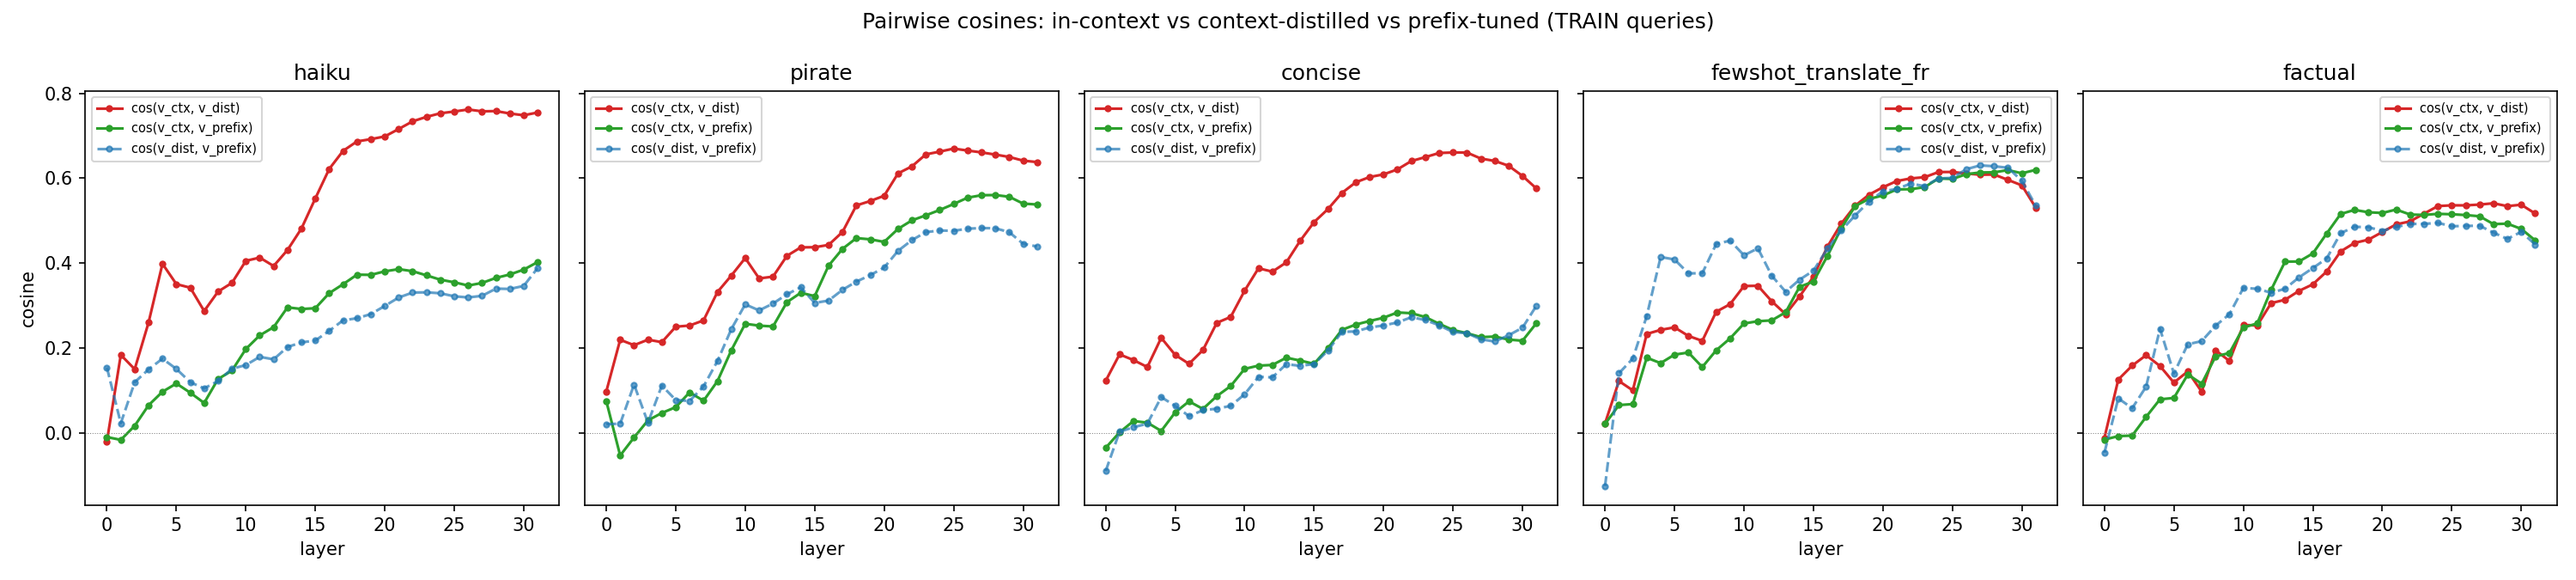
\includegraphics[width=\linewidth]{figures/fig_prefix_cos_train.png}
\caption{Pairwise cosine similarities between $v^\text{ctx}$ (in-context)
and the perturbations from full distillation $v^\text{dist}$ and prefix
tuning $v^\text{prefix}$. Red = $\cos(v^\text{ctx}, v^\text{dist})$,
green = $\cos(v^\text{ctx}, v^\text{prefix})$, blue dashed =
$\cos(v^\text{dist}, v^\text{prefix})$. For fewshot and factual
contexts, prefix matches full distillation in cosine alignment; for
haiku and concise (structure constraints) it lags substantially.}
\label{fig:prefix_cos}
\end{figure}

\paragraph{Activation alignment is mixed.}
Figure~\ref{fig:prefix_cos} shows the three pairwise cosines per layer.
For \emph{knowledge-like} contexts (fewshot translation, factual
injection), the prefix achieves cosine alignment with $v^\text{ctx}$
that matches or exceeds full distillation
($\cos = 0.62$ for fewshot, vs $0.62$ for distill;
$\cos = 0.53$ for factual, vs $0.54$). For \emph{constraint-like}
contexts (haiku, concise, pirate), the prefix's alignment
($0.28$--$0.56$) lags behind full distillation ($0.66$--$0.76$).

This makes sense mechanistically: prefix tuning provides extra K/V
tokens for attention to read, which is well-suited to ``additional
content to retrieve'' (a fact, a translation example) but poorly suited
to ``a constraint on output form'' (5-7-5 haiku, one-sentence answers,
pirate vocabulary). The structure-constraint contexts seem to need
the model's output computation itself to change, which prefix tuning
does not allow.

\begin{table}[t]
\centering
\caption{MMLU-Pro accuracy comparison including prefix-tuned model.
Prefix tuning, despite using only~$\approx 1$\,M trainable parameters,
does \emph{not} preserve general capability. For the haiku context in
particular, prefix tuning collapses MMLU-Pro from~$0.36$ to~$0.07$ ---
worse than full distillation's preserved~$0.37$.}
\label{tab:mmlu_prefix}
\small
\begin{tabular}{lccccc}
\toprule
Context & base & in-context & context-distilled & prefix & $\Delta$prefix \\
\midrule
haiku                  & 0.360 & 0.295 & 0.365 & 0.070 & $\mathbf{-0.290}$ \\
pirate                 & 0.360 & 0.325 & 0.125 & 0.145 & $-0.215$ \\
concise                & 0.360 & 0.380 & 0.300 & 0.085 & $\mathbf{-0.275}$ \\
fewshot\_translate\_fr & 0.360 & 0.375 & 0.135 & 0.135 & $-0.225$ \\
factual                & 0.360 & 0.320 & 0.140 & 0.125 & $-0.235$ \\
\bottomrule
\end{tabular}
\end{table}


\paragraph{But MMLU-Pro accuracy is destroyed too.}
Table~\ref{tab:mmlu_prefix} reports MMLU-Pro accuracy with the
prefix-tuned model added as a fourth variant. The result is striking:
\textbf{prefix tuning destroys MMLU-Pro accuracy for every context, in
some cases more severely than full distillation.} For haiku, the
prefix-tuned model crashes from~$0.36$ to~$0.07$ --- below the random
baseline that one might expect from the floor of a 10-option MCQ.

This is the mechanism we missed. Even though the prefix preserves the
structure of ``extra K/V for attention to read,'' the model has been
\emph{trained} to use the prefix to produce context-specific outputs.
At inference time on out-of-distribution queries, the prefix is still
active in every attention layer, and the model has lost the ability to
ignore it. Selectivity is broken not by the K/V's existence but by the
training signal that conditioned the model on its presence.

\paragraph{Diagnosis: bake-in is the problem.}
Both full distillation and prefix tuning train the model to act
context-conditioned given $C$'s effect, with $C$ no longer in the
input. Once trained, the model cannot tell when $C$ is supposed to
apply --- it always does. In-context preserves selectivity because
$C$ is in the input itself: the model's attention to $C$'s tokens
naturally drops when the rest of the prompt makes $C$ irrelevant.
The lesson is that ``bake the context into the weights/parameters''
is not the right primitive for context compression. A correct
solution would need either (a) a content-conditional gate on whether
to apply the absorbed context, or (b) keeping the context's tokens
in the input but compressed (e.g., a learned summary token), so that
attention retains its selectivity. Both are open directions for future
work.

\section{Related work}
\label{sec:related}

\paragraph{In-context learning as implicit gradient descent.}
\citet{vonoswald2023transformers}, \citet{akyurek2023learning}, and
\citet{garg2022what} establish, in linear- or restricted-attention
settings, that a forward pass over an in-context demonstration is
mathematically equivalent to one step of gradient descent on a
meta-objective. They characterise what in-context is doing internally,
without ever performing the explicit gradient descent on the real
transformer's weights. Our work runs the empirical sibling experiment:
context-distillation \emph{actually} performs gradient descent on the
model's weights and we measure how close the resulting activation
pattern is to the in-context one. The peak cosine of $0.42$--$0.80$
supports the qualitative prediction on a real instruction-tuned
transformer, but the magnitude gap (context-distilled overshooting
in-context by a factor that grows with depth) shows the empirical
equivalence is directional, not exact.

\paragraph{Knowledge editing.}
ROME~\citep{meng2022rome} and MEMIT~\citep{meng2023memit} edit weights to
inject specific facts. Our factual-context experiment is the dual
operation: rather than choosing the edit, we let SGD discover one and
ask whether the result resembles the context that prompted it.

\paragraph{Soft prompts and prompt distillation.}
Soft-prompt tuning~\citep{lester2021power} treats context as a learned
embedding; prompt distillation~\citep{askell2021general} compresses long
prompts into shorter ones via supervised fine-tuning. The latter is
methodologically close to our distillation step, but it is consumed as a
training procedure, not as a mechanistic probe.

\section{Discussion}
\label{sec:discussion}

\paragraph{Same direction, different amount.}
In-context and context-distilled produce \emph{aligned but not
identical} residual-stream perturbations. The cosine reaches
$0.42$--$0.80$ in late layers, but $\|v^\text{dist}\| > \|v^\text{ctx}\|$
at every layer with the gap widening with depth. The two interventions
are related but not interchangeable.

\paragraph{Bake-in fails regardless of capacity.}
The MMLU-Pro and prefix-tuning experiments reveal a deeper structural
issue: \emph{any} fine-tune that compresses $C$ into model parameters
--- whether 8\,B parameters of full FT or 1\,M parameters of prefix
K/V --- destroys general capability on unrelated tasks, often more
severely than the smaller-parameter approach. The shared failure
mode is the bake-in itself: the absorbed context is always active on
every forward pass, with no mechanism for the model to recognise
when it is irrelevant. In-context preserves capability because
attention can choose to ignore $C$'s tokens based on the rest of the
input. Whatever the right primitive for ``compressing context into
model memory'' is, it is not bake-in.

\paragraph{Implications for the in-context-learning-as-GD literature.}
The line of work from \citet{vonoswald2023transformers} and follow-ups
predicts that explicit GD on a suitable meta-loss should match the
in-context forward pass. Our cosine of $0.42$--$0.80$ is consistent with
that prediction extended to a real 8B transformer with a real CE loss;
the gap from~$1.0$ and the magnitude overshoot together suggest either
that real CE-on-tokens is not exactly the meta-loss those papers
identify, or that 32 nonlinear layers leave many descent directions
equivalent for the same behavior --- and SGD picks one that goes
\emph{further} along that direction than the in-context computation does.

\paragraph{Why magnitudes diverge.}
We do not have a complete account, but a plausible reading is that
context-distillation is trained to reproduce specific outputs, so
gradient pressure does not stop once the right direction is found ---
it continues until the loss is minimised. In-context, by contrast, is
the result of a single forward pass that has no such optimisation
pressure: it produces just enough perturbation to elicit the
context-conditioned behavior. Two routes to similar outputs, with
different stopping points.

\section{Limitations}
\label{sec:limitations}

\begin{itemize}
\item Single model family (Llama-3.1-8B-Instruct). Whether the
  in-context vs context-distilled comparison transfers to other
  architectures is open.
\item Single training-set size, learning rate, and step count per
  context. Whether the magnitude overshoot persists with longer
  training, more data, or different optimisers is open.
\item The synthetic distillation set is generated by the same base
  model that is being fine-tuned, so context-distilled is closer to
  behavior cloning of self-outputs than to imitation of an external
  teacher; results may underestimate the difficulty of context
  internalisation in general.
\item We do not perform any weight-space comparison. The paper claims
  pertain only to activations.
\item Single run per (context) configuration. No error bars across
  seeds or training-recipe variations.
\item Probe and validation sets are small ($\approx 30$ queries
  each); a downstream-task benchmark would tighten the behavioral
  claim.
\end{itemize}

\bibliography{references}

\newpage

\end{document}
